The value in the resampling process above largely lies in the ability to present well-defined document prototypes to a resampling process.  There are many potential sources for document retrieval according to this prototype, including the original input corpus, a separate `super-corpus', or, ideally a separate population (that is itself not a sample).

The proof-of-concept evaluated here implements a number of web-based retrieval mechanisms that are designed around search methods already used in tools such as BootCaT~\td{cite}.  As with the original sample design, these retrieval methods are designed to be selectable by the end user: in the simplest case, using only the `Bing' search engine~\td{cite/footnote} would result in a very similar sampling method to that used in BootCaT itself, yet also yield statistics regarding the error of the retrieval mechanism.  This is analogous to being able to gauge measurement error.

This process is deliberately agnostic of any internal variables: the \textsl{content} of the retrieved texts is also affected by the choice of retrieval mechanism, however, this is part of the variance desired in the dataset, and should form part of any motivating research question.

The problem of when the output corpus is `sufficiently large' may not be solved using this method: whilst the convergeance of the output corpus to the input is known to some degree of certainty, the same cannot be said of the errors in retrieval.  Assuming that each text is entirely accurate to its prototype will yield a corpus showing the same distribution as the input, but this does not mean that the source used is presenting data in an unbiased manner, or that sufficient variation has been captured to generalise about \textsl{that} population.

It is also possible to select documents that are not a perfect fit to the prototype: indeed, this may be necessary where continuous measures are used to characterise the sampling design.  In this case, the residual variation may be used to determine bias in the selection method by measuring how non-uniform the distribution of these residuals is.  Note, however, that even uniform nonzero residuals represent an overall increase in dispersion compared to the input distribution: it is almost certainly more useful to deliberately apply this to the input distribution by applying a smoothing method prior to resampling than it is to rely on the document retrieval stage (which may apply said dispersion in less predictable ways).

\til{
further work:\\
Though not implemented here, it is possible to use this known error distribution as a correction mechanism for the sampler, deliberately seeking to `shore up' the residuals.  This kind of feedback loop is used in bootstrapping algorithms such as Gibbs and slice sampling, though its application to a procedure based on a fairly hard-to-predict search mechanism (web search engines) presents major engineering challenges.
}

% --


\begin{figure}[Ht]
    % ./analysis/loglik-significance.r
    \centering
    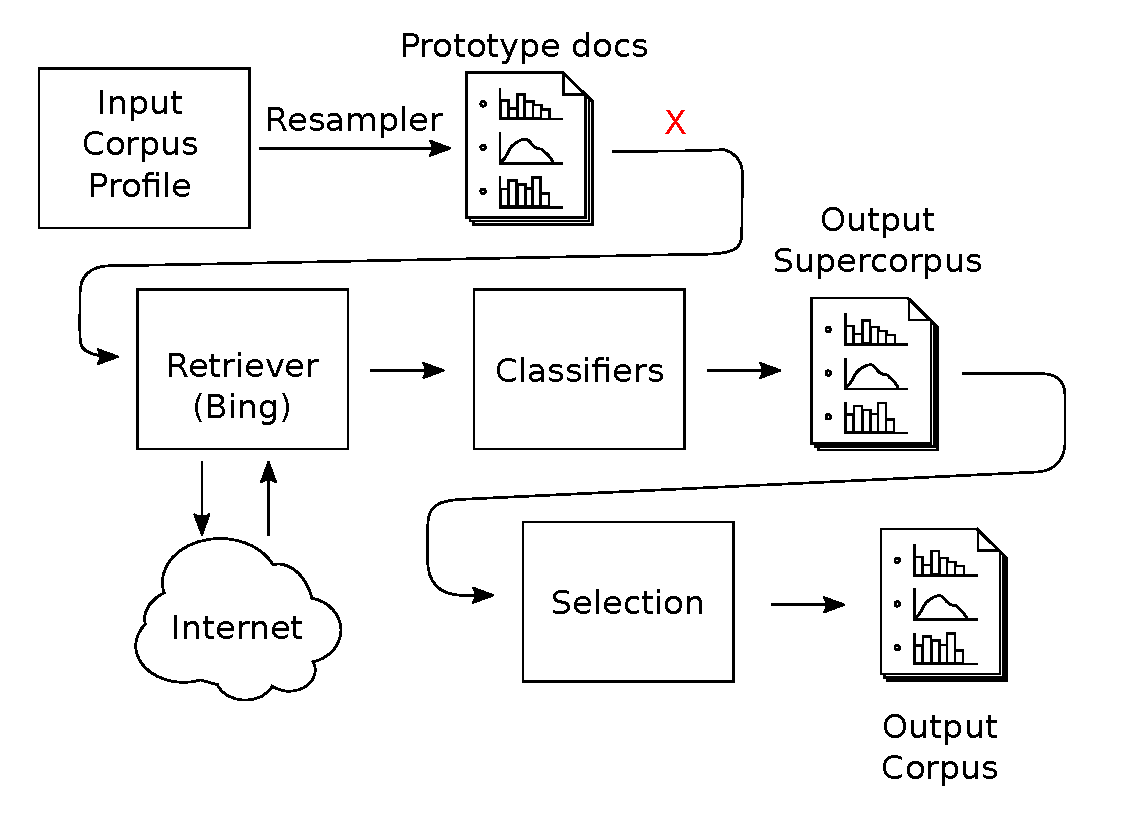
\includegraphics[width=0.8\textwidth]{evaluation/retrieval-overview}
    \caption{An overview of the retrieval mechanism used in the proof-of-concept implementation.}
    \label{fig:evaluation:retrieval:outline}
\end{figure}



The retrieval method used here (outlined in Chapter~\ref{sec:rebuilding} and Figure~\ref{fig:evaluation:retrieval:outline}) is based on the principle of heuristically seeking documents fitting the prototype, followed by a ranking stage and selection of the highest-ranked document.  This means that it has the potential to output imperfect documents but is maximally unlikely to do so.  It does not adjust for any accumulated error during execution, so has the potential to gradually accumulate errors in one particular direction if `perfectly matched' documents are not available within the parameters given.  This approach is largely taken to prevent the retriever from searching endlessly for a combination of metadata values that simply do not exist in the sources to which it has access: many specific uses of this technique will be able to use far more certain methods for their retrieval stage (up to and including manual selection of documents).



\subsection{Method}
\label{sec:evaluation:method}





\subsection{Data}
\label{sec:evaluation:method}
Discuss which corpora were chosen and why

\subsection{Results}
\label{sec:evaluation:}
Provide quantitative measures for the two evaluation methods
%#\subsubsection{Partial/white box}
%Show how well classifiers and heuristics behave
\subsubsection{Complete/black box}
Show how well the whole system works

